\section{Nebenläufigkeit, Transaktionen}
\label{sec:parallel}

\textbf{Transaktion}
\begin{items}
	\item Partiell geordnete Folge von Lese- und Schreibzugriffen auf Datenobjekte (mit Commit oder Abort am Ende)
	\item \underline{ACID Eigenschaften:}
	\item Atomicity: Entweder alles oder gar nichts ausführen
	\item Consistency: Integritätsbedingungen bleiben erhalten
	\item Isolation: Nutzer hat Eindruck, er wäre alleine
	\item Durability: Änderungen sollen dauerhaft sein
\end{items}

\textbf{Synchronisation}
\begin{items}
	\item Viele Nutzer sollen Daten gleichzeitig lesen und schreiben können
		\\*
		\( \leadsto \) Konsistenz sicherstellen \( \leadsto \) \textbf{Synchronisationskomponente}
	\item \underline{Serielle Ausführung}: 
		\\*
		+ Konsistenz immer gewährleistet 
		\\*
		$-$ extreme Wartezeiten, schlechte Ressourcenausnutzung
\end{items}

\textbf{Unkontrollierte nicht-serielle Ausführung: Probleme}
\begin{items}
	\item \textbf{Lost Update}\\
		 Programm \( T_1 \) transferiert 300 EUR von Konto \( A \) nach \( B \),
		\\*
		Programm \( T_2 \) schreibt Konto \( A \) \( 3 \% \) Zinsen gut
		\\*
		\( \leadsto \) Zinsen aus \( S_5 \) von \( T_2 \) verloren, weil \( T_1 \) in \( S_6 \) überschreibt

	\begin{figure}[H]\centering\label{Synchronisation}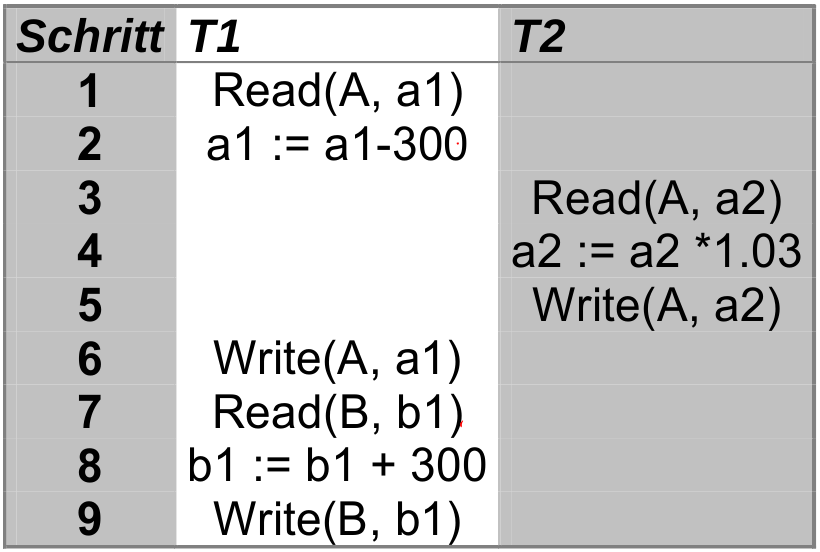
\includegraphics[width=0.2\textwidth]{Synchronisation}\end{figure}
	
	\item \textbf{Dirty Read}\\
		Commit, Abort \\
		\( T_2 \) schreibt Zinsen gut basierend auf einem Wert, der nicht zu einem konsistenten Zustand gehört, denn später erfolgt Abort von \( T_1 \)

	\begin{figure}[H]\centering\label{DirtyRead}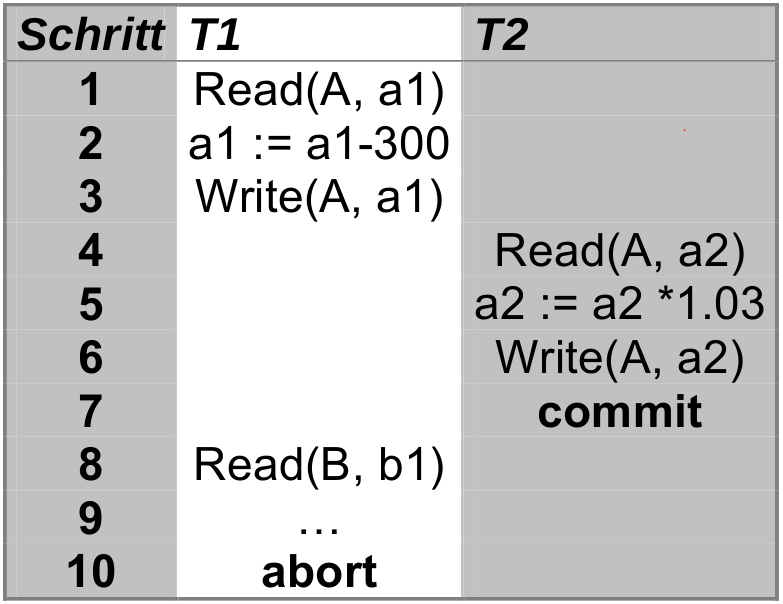
\includegraphics[width=0.2\textwidth]{DirtyRead}\end{figure}
	
	\item \textbf{Non-Repeatable Reads}\\
		 Programm liest Datenobjekt mehr als einmal und sieht dabei Änderung durch anderes Programm
	\begin{figure}[H]\centering\label{NonRepeatableRead}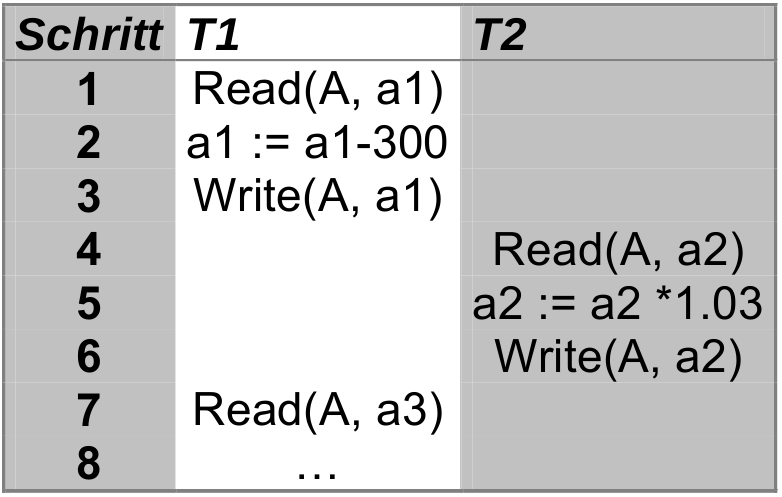
\includegraphics[width=0.2\textwidth]{NonRepeatableRead}\end{figure}
	
	\item \textbf{Phantom}\\
		Berechnung von Änderung auf veralteten Werten
\end{items}

\textbf{Konflikt}
\begin{items}
	\item Zwei Operationen \( p, q \) konfligieren
		\\*
		\( \Leftrightarrow \) \( p,q \) greifen auf selbes Datenobjekt zu und \( p \) oder \( q \) ist Schreiboperation
	\item In einer Transaktion müssen konfligierende Operationen \textbf{geordnet sein} (andere nicht zwingend)
\end{items}

\textbf{Histories}
\begin{items}
	\item \underline{Vollständige Historie}: Menge von Transaktionen und Ausführungsordnung (nebenläufige Verzahnung, Ordnung konfligierender Operationen zwischen Transaktionen)
	\item \underline{Historie}: Präfix einer vollständigen Historie
	\item \underline{Commited Projection} (\( C(H) \)): H nach Entfernen aller nicht-committeten Operationen
	\item Eine Eigenschaft von Histories ist \textbf{prefix commit closed}
		\\*
		\( \Leftrightarrow \) (\( H \) erfüllt Eigenschaft \( \Rightarrow C(H') \) erfüllt Eigenschaft)
\end{items}

\textbf{Konfliktäquivalenz (CSR)}
\begin{items}
	\item \( H, H' \) (Konflikt-)Äquivalent, wenn
	\begin{enumeration}
		\item gleiche Transaktionen, gleiche Operationen
		\item gleiche Ordnung konfligierender Operationen (gleiche Konfliktrelation)
	\end{enumeration}
\end{items}

\textbf{Serialisierbarkeit}
\begin{items}
	\item \( H \) serialisierbar \( \Leftrightarrow C(H) \equiv H_S \) (serielle History)
	\item \underline{Serialisierbarkeitsgraph} (Abhängigkeitsgraph):
		\\*
		Knoten = Transaktionen
		\\*
		(gerichtete) Kante von $T_1$ nach $T_2$ wenn $op_1$ und $op_2$ konfligieren und $op_1 < op_2$
	\item \textbf{Theorem}: Schedule ist serialisierbar, wenn entsprechender Abhängigkeitsgraph zykelfrei ist
	\item Konflikt-Serialisierbarkeit ist prefix commit-closed
	\item \textbf{Ansatz nicht praktikabel}:
	\begin{enumeration}
		\item Serialisierbarkeit nur im Nachhinein überprüfbar
		\item Administrativer Overhead zu hoch: Abhängigkeiten zu bereits terminierten Transaktionen berücksichtigen
	\end{enumeration}
\end{items}

\textbf{Rücksetzbarkeitsklassen}
\begin{items}
	\item \underline{Rücksetzbar (RC)}: Commit für $T_j$ erst erlaubt, wenn alle $T_i$ von denen $T_j$ liest, committed sind (Abort darf Semantik von bereits committeten Transaktionen nicht verändern).
	\item \underline{Avoid cascading aborts (ACA)}: Nur Objekte von bereits committeten Transaktionen lesen.
	\item \underline{Striktheit (ST)}: Objekte von noch nicht committeten Transaktionen dürfen weder gelesen noch überschrieben werden (ermöglicht einfache Implementierung des Rücksetzens)
\end{items}

\textbf{Locking}
\begin{items}
	\item Lock für jedes Datenobjekt und jede Operationsart
		\\*
		Notation: \( rl_i[x] \), \( wl_i[x] \)
	\item Aber: Sperrdisziplin alleine reicht für Korrektheit nicht aus!
	
	\item \textbf{Zwei-Phasen-Sperrprotokoll (2PL)}:
	\begin{enumeration}
		\item Locks werden hinzugenommen
		\item Locks werden freigegeben
	\end{enumeration}
	\( \leadsto \) Serialisierbarkeit sichergestellt\\
						Deadlocks sowie kaskadierende Abbrüche weiterhin möglich
	
	\item \textbf{Strenges Zwei-Phasen-Sperrprotokoll (S2PL)}: 
	
	Atomare Freigabephase am Ende der Transaktion\\
	\( \leadsto \) Zusätzlich ACA: Vermeidung kaskadierender Abbrüche
	
	\item \textbf{Konservatives Zwei-Phasen-Sperrprotokoll (C2PL)}:
	
	Atomare Anforderungsphase zu Beginn der Transaktion\\
	\( \leadsto \) Zusätzlich: Vermeidet Deadlocks
	
	\item \textbf{CS2PL}: 
	
	Kombination aus streng und konservativ: Atomare Anforderungs- und atomare Freigabephase \\
	\( \leadsto \) Serialisierbarkeit, ACA, Deadlockfreiheit
	
	\item \textbf{Aber:} Jede Einschränkung schränkt auch die Zahl der möglichen Histories ein und verringert damit den möglichen Grad der Parallelität!
	
\end{items}

\begin{fragen}
	\begin{enumeration}
		\item Was ist Isolation? Was ist der Zusammenhang zwischen Isolation und Serialisierbarkeit?
		\item Welche Probleme können bei unkontrollierter nebenläufiger Ausführung von Transaktionen auftreten?
		\item Beispiele für Lost Updates, Non-Repeatable Reads usw. angeben, die bestimmte Bedingungen erfüllen
		\item Warum ist es wichtig, dass unser Korrektheitskriterium für Histories prefix commit closed ist? Erklären Sie, warum Konflikt-Serialisierbarkeit prefix commit closed ist.
		\item Ist eine gegebene History serialisierbar/recoverable/cascadeless?
		\item Haben zwei Konflikt-äquivalente Histories stets die gleichen Reads-from-Beziehungen?
		\item Warum verwendet man in der Regel nicht den Serialisierbarkeitsgraphen, um Serialisierbarkeit sicherzustellen?
		\item Bei Deadlocks wird in der Regel eine Transaktion zurückgesetzt. Kann es vorkommen, dass die gleiche Transaktion mehrmals/beliebig oft zurückgesetzt wird? Wenn ja, was kann man jeweils dagegen tun?
		\item Geben Sie ein Beispiel für eine serialisierbare Ausführung, bestehend aus drei Transaktionen, mit folgender Eigenschaft an: Die zeitliche Reihenfolge der Commits ist \( c_1 \) vor \( c_2 \) vor \( c_3 \), die der äquivalenten seriellen Ausführung jedoch \( c_3 \) vor \( c_2 \) vor \( c_1 \).
		\item Um einen Deadlock aufzulösen muss eine der beteiligten Transaktionen zurückgesetzt werden. Welche Kriterien sind Ihres Erachtens nach sinnvoll, um diese Auswahl zu treffen?
	\end{enumeration}
\end{fragen}